\chapter{CONCEITOS BÁSICOS\textbf{}}
\label{chp:capitulo2}

Nesse capítulo busca-se elucidar as principais terminologias, técnicas, algoritmos e tecnologias no geral que estão relacionadas a esse trabalho, realizando-se um apanhado geral e exemplificando alguns casos de uso desses assuntos.

\section{SQL Injection}

O tipo mais comum e mais prevalecente de injeção de código é o de \textit{SQL Injection}, que manipula bancos de dados via \verb+SQL+ (\textit{Structured Query Language}), a linguagem clássica de manuseio de bancos de dados, para receber acesso a informações sensíveis.

Exemplificando algumas situações de SQL Injections \cite{sql_port_swigger}:

\begin{alineas}
    \item 
    Consideremos uma aplicação que possui uma funcionalidade básica de login, com usuário e senha. Quando o usuário fornece as entradas \verb+‘usuário'+ e \verb+'123’+ como credenciais, a seguinte query SQL é realizada pelo sistema na checagem:
    
    \begin{verbatim}
        SELECT * FROM users 
        WHERE username = ‘usuario’ AND password = ‘123’
    \end{verbatim}
    
    Caso o usuário e senha sejam iguais a um registro na base de dados, todas as colunas da tabela \verb+user+ serão retornados. Caso contrário, os dados não serão obtidos.
    Nesse caso, se o atacante usa a sequência de comentário SQL \verb+--+, ele é capaz de remover a checagem de senha da cláusula \verb+WHERE+.
    A sequência de caracteres \verb+--+ representa comentário em SQL. Caso a aplicação não tenha uma higienização dos dados, é possível inserir esses caracteres como entrada e serão processados como uma instrução na query. Por exemplo, se no parâmetro que é o \verb+username+ da consulta for inserido \verb+administrator’--+ e uma senha em branco, a seguinte query é processada:
    
    \begin{verbatim}
        SELECT * FROM users 
        WHERE username = 'administrator'--' AND password = '' 
    \end{verbatim}
    
    Isso efetivamente retorna o usuário cujo \verb+username+ é \verb+administrator+ e realiza o login do atacante como tal, expondo funções sensíveis da aplicação web inteira.

\end{alineas}

\begin{alineas}
    \item
    Em uma aplicação de e-commerce que organiza produtos em categorias diferentes, podemos ter um caso onde o usuário clica em uma categoria \verb+‘Presentes’+, requisitando o seguinte URL do navegador web:
    
    \textbf{https://insecure-website.com/products?category=Presentes}
    
    Isso faz com que a aplicação realize uma query SQL para resgatar detalhes de tais produtos do banco de dados:
    
    \begin{verbatim}
        SELECT * FROM products
        WHERE category = ‘Presentes' AND released = 1 
    \end{verbatim}
    
    Tal query retorna todos os detalhes (identificado por \verb+*+) da tabela de produtos, onde a categoria é \verb+‘Presentes’+ e a restrição \verb+released+ é 1. Essa restrição, quando observada por um atacante astuto, se revela como algo usado para esconder produtos não lançados. Esse atacante pode então construir um ataque digitando a seguinte URL, dado que o site não previne contra ataques SQL:
        
    \textbf{https://insecure-website.com/products?category=Presentes’--}
    
    Que provoca a seguinte query SQL:
    
    \begin{verbatim}
        SELECT * FROM products 
        WHERE category = 'Presentes'--' AND released = 1 
    \end{verbatim}
    
     Uma vez que a sequência \verb+--+ anteriormente vista denota um comentário SQL, a parte depois de 
    \verb+‘Presentes’+ é interpretada como tal e não é executada, revelando todos os produtos escondidos.

\end{alineas}

\begin{alineas}
    \item
    Também é possível recuperar dados de outras tabelas de um banco de dados, utilizando a \textit{keyword} \verb+UNION+ \cite{mysql_union}, que combina o resultado de múltiplas consultas \verb+SELECT+ em apenas um conjunto. Se um atacante executa a seguinte query contendo a entrada de usuário \verb+`Presentes`+, ainda no último exemplo de site:
    
    \begin{verbatim}
        SELECT name, description
        FROM products WHERE category = ‘Presentes'
    \end{verbatim}
    
    Então ele pode também submeter uma entrada nociva com \verb+UNION+:
    
    \begin{verbatim}
        ' UNION SELECT username, password FROM users--
    \end{verbatim}
        
    Tal entrada faz com que todos os usuários e senhas venham juntos das descrições dos supostos presentes, fundamentalmente comprometendo a segurança da aplicação

\end{alineas}


No contexto deste trabalho, no entanto, é estudado uma forma tanto comercial como \textit{open-source}  que têm tido crescimento no mercado: o uso de \textit{Web Application Firewalls}, mais especificamente os baseados em técnicas de Aprendizado de Máquina.

Forma de ataque ampla onde uma entrada de dados recebe caracteres não tratados que são executados pelo sistema com objetivo de alterar o funcionamento padrão do software.
Além dos exemplos bases de injeção SQL, existem variantes \cite{bach_owasp2020understanding} do SQL Injection como: \textit{error-based, union-based, blind} e \textit{out-of-band} \cite{out_of_band_sql_invicti}. \textit{Error-based} são injeções que fornecem erros de SQL para o atacante, vazando informações críticas do banco de dados. \textit{Union-based} são ataques que utilizam uma query existente na lógica do sistema concatenada a outra através de um \verb+UNION+ de maneira a executar uma segunda lógica além da já estabelecida pelo sistema. Injeções às cegas (\textit{blind-based}) são aquelas que o sistema não dá nenhuma informação após a injeção, de forma que o atacante precisa ser engenhoso para obter informações e prosseguir com a ofensiva. \textit{Out-of-band} é uma injeção sem o fornecimento de uma saída para o atacante, porém é possível redirecionar a saída para um endpoint, geralmente servidor http.
É fundamental para mitigar as injeções ter uma validação dos caracteres e declarações válidas ao receber uma entrada de dados na aplicação web.

Injeção (em especial SQL) é uma das vulnerabilidades mais comuns, de baixa complexidade para o atacante e historicamente impactante, o que motivou o trabalho em aprofundar em um problema subestimado por desenvolvedores, que tem impactos profundos na confiabilidade, integridade e disponibilidade de um serviço web.

\section{Cross Site Scripting, ou XSS}
\textit{Cross Site Scripting} é uma técnica conhecida como XSS onde geralmente há uma injeção de \textit{scripts} maliciosos na aplicação web, revelando dados sensíveis, serviços internos ou divulgação de \textit{cookies} de usuários com privilégios.
Existem três variantes de XSS: \textit{stored} XSS, onde o atacante injeta um \textit{payload} no servidor web, de maneira que quando outro usuário faz a requisição para acessar a página, o \textit{payload} é ativado. Outro caso é o de \textit{Reflected} XSS, quando o atacante injeta dados através de um método HTTP gerando uma resposta imediata na aplicação. Este permite o malfeitor forjar uma URL específica que ao ser acessada pela vítima vaza dados sensíveis, como \textit{cookies}. E por último a variante \textit{DOM Based} XSS que consiste na inserção de código malicioso no DOM (\textit{Document Object Model}), sem refletir no código-fonte HTML, sendo ativado apenas pelo console DOM.
Dados obtidos de fontes não confiáveis devem ser devidamente validados e normalizados para evitar XSS.

Um dos \textit{Web Application Firewalls} mais utilizados na solução proposta também oferecia avaliação para ataques XSS, sendo importante compreender qual tipo de vulnerabilidade é analisada em determinadas seções do código.


\section{Algoritmos de Fuzzing}

O cerne do algoritmo por trás do \textit{WAF-A-MoLE} e o \textit{wafamole++} se encontra na técnica de \textit{fuzzing}. O termo \textit{fuzz} foi cunhado pelo professor da Universidade de Wisconsin-Madison Barton Miller nos anos 80, após sofrer uma interferência considerável de uma tempestade no funcionamento de aplicações que rodavam em um ambiente \textit{unix} remoto na época \cite{fuzzing_info}. 

Pouco depois disso o mesmo passou aos seus alunos uma tarefa denominada o \textit{"Fuzz Generator"}, na qual era necessário implementar uma ferramenta que testasse a robustez de programas \textit{unix} através de um bombardeio de informações aleatoriamente geradas.

Atualmente é uma técnica amplamente aceita na testagem/sondagem da segurança de diversas aplicações, com um leque de ofertas de \textit{fuzzing} comerciais no mercado. E naturalmente é empregável em \textit{Web Application Firewalls}, permitindo extrair informações valiosas que rendam aprimoramentos para os mesmos. Enquanto a idéia em si de \textit{fuzzing} permanece a mesma, as maneiras de efetuá-lo tiveram um grande progresso de mudança.


Uma função elementar de \textit{fuzzing} pode ser vista abaixo:

\includecode[C]{Função de um \textit{fuzzer}  elementar} {alg:codigo1}{codigos/fuzzer.py}

\bigskip
Tais funções de \textit{fuzzing} podem ser aprimoradas, customizadas para testar os mais diversos programas. Uma das maneiras de polir os resultados oriundos de \textit{fuzzing} elementar, que podem ser rejeitados facilmente por muitos programas inicialmente, é um processo chamado \textit{fuzzing} mutacional, ou \textit{mutational fuzzing}, projetado para melhorar as chances de obter entradas consideradas válidas.

Nessa estratégia, a execução se inicia com uma entrada válida, e ela subsequentemente sofre uma mutação pequena, como no caso de uma string a mudança de um caractere, adição/remoção de um número, ou até mesmo uma troca de um bit (todos naturalmente aleatórios, pelo princípio do funcionamento de \textit{fuzzing}).

\includecode[C]{Classe de \textit{fuzzer} mutacional} {alg:codigo1}{codigos/mutational_fuzzer.py}

\bigskip
O programa acima realiza, dentre três operadores de mutação, uma mutação aleatória ao chamar a função \verb+mutate()+. Na prática, são realizadas uma série de mutações para que se produzam entradas viáveis. Com um simples \textit{loop} para chamar a função \verb+mutate()+ isso é possibilitado.

Essas técnicas geralmente encontram \textit{bugs} de corrupção de memória simples e a aleatoriedade, dispersão fazem com que a eficiência do ataque seja baixa, além de cobrir poucas partes do código. Por outro lado, é simples de implementar, tem boa extensibilidade e pode ser feita sem o código-fonte. O \textit{fuzzing} aumenta seu potencial quando o alvo está em execução em um ambiente real. Outro ponto positivo é o fato de poder aplicar a técnica em aplicações com pouco conhecimento prévio sobre.

Em suma \textit{fuzzing} consiste na geração massiva de entradas normais e anômalas para uma aplicação específica, seguido da detecção de exceções no algoritmo devido o processamento das entradas geradas e monitoramento dos estados de execução da aplicação. Quando comparado com outras técnicas como análise estática, dinâmica e execução simbólica, o \textit{fuzzing} apresenta facilidade em ser implementado, boa precisão (em ambientes reais) e boa escalabilidade.

Expandindo um pouco o conceito, um teste de \textit{fuzzing} tipicamente consiste na geração em larga escala de entradas para um programa específico, entradas conhecidas também como \textit{testcases}. A qualidade de tais \textit{testcases} criados influencia diretamente na qualidade do teste fuzzing. As entradas precisam atender os requisitos do programa testado para o padrão de entrada. Em contrapartida, as entradas precisam ser errôneas o suficiente para gerarem falhas ou erros no processamento do programa. De acordo com o alvo, as entradas podem ser arquivos com diferentes formatos, dados de comunicação entre redes, binários executáveis específicos, entre outros. No caso do \textit{wafamole++} trabalha-se, conforme descrito anteriormente, com injeções SQL.

Gerar \textit{testcases} suficientemente errôneos é uma tarefa árdua, com duas variantes: \textit{generation-based} e \textit{mutation-based}, das quais a última é a adotada pelo \textit{WAF-A-MoLE} e \textit{wafamole++}. Depois de gerados, os \textit{testcases} alimentam o programa alvo, tendo variáveis de ambiente e outros parâmetros do software a ser testado devidamente configurados pelo programador. Geralmente um teste de \textit{fuzzing} tem como condição final um tempo limite (ou \textit{timeout}) pré-definido ou uma falha de execução do programa.

\textit{Fuzzers} monitoram o estado de execução durante o processo, aguardando exceções ou falhas.  Formas comuns de metodologia de monitoramento de exceções incluem monitor sinais específicos do sistema, falhas e outras violações. Existem ferramentas para verificar comportamentos anormais difíceis de perceber intuitivamente, como o \verb+AddressSanitizer+, \verb+DataFlowSanitizer+, \verb+ThreadSanitizer+ e \verb+LeakSanitizer+. Quando uma violação é capturada, o \textit{fuzzer} armazena o \textit{testcase} que a causou para análise futura e replicação \cite{li2018fuzzing}.

Por fim, na fase de análise, tem-se por objetivo determinar a localidade e a causa da violação no software. A análise geralmente é feita com o auxílio de \textit{debuggers} como \verb+DGB+, \verb+windbg+ ou outras ferramentas de análise binária, como a \verb+IDA Pro+, \verb+OllyObg+ e outras. O exato estado de execução dos \textit{testcases}, informações da \textit{thread}, instruções e outras informações fazem parte do monitoramento. Para o caso do trabalho em questão, considerando-se o ambiente em \textit{Python}, o \textit{debugger} padrão \verb+pdb+ mostrou-se suficiente para diagnosticar a maioria dos \textit{bugs} encontrados.

\begin{figure}[ht]
    \centering
    \caption{Workflow Fuzzing}
    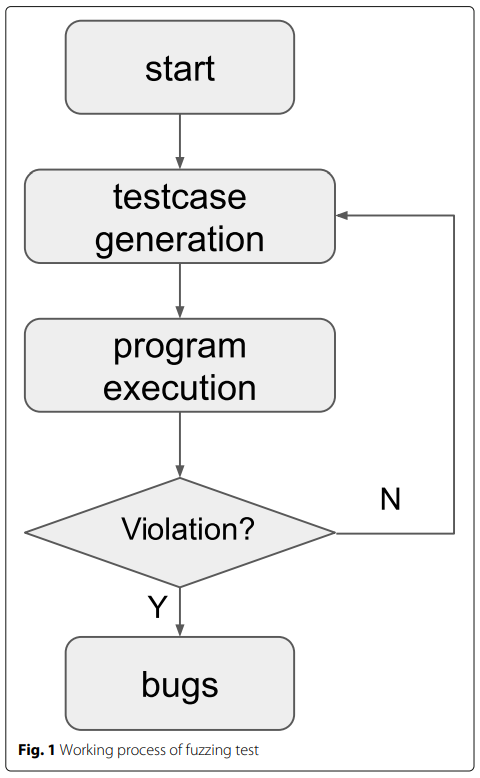
\includegraphics[width=8cm,height=12cm,keepaspectratio]{figuras/fuzzing imagem.png} 
    \legend{Fonte: \href{https://parsif.al}{Fluxograma} (2022, p. TO-DO)}
    \label{fig:internet} 
\end{figure}

O \textit{fuzzer} \textit{generation-based} necessita saber como é a entrada que o programa é capaz de processar. No caso de um \textit{fuzzing} para arquivos, geralmente é fornecido um arquivo de configuração com o modelo pré-definido de entrada. Os \textit{testcases} são gerados de acordo com o arquivo de configuração. Fuzzers desse tipo tem facilidade em burlar validações do software testado, permitindo ao pentester entender com mais profundidade a aplicação estudada. Por outro lado, sem uma documentação amigável, analisar o formato do arquivo pode ser uma tarefa árdua.
Em termos de praticidade, fuzzers mutation-based são mais fáceis de utilizar, com aplicabilidade genérica, sendo geralmente o tipo adotado por testes de intrusão no estado da arte. Diferente do generation-based, o mutation-based precisa de algumas entradas iniciais válidas. As entradas vão sofrendo mutações e novos \textit{testcases} vão sendo gerados. O \textit{wafamole++} requer apenas uma entrada inicial válido - uma query que é fornecida ao final de cada chamada ao comando \verb+wafamole evade+.

Para testes \textit{grey box} e \textit{black box}, os \textit{fuzzers} são \textit{mutation-based}. Para testes \textit{white box}, \textit{generation-based}.

O contexto relevante para o \textit{WAF-A-MoLE} é produzir, iterativamente, múltiplas injeções SQL a serem testadas a cada "rodada" de mutação. Uma injeção SQL é usada como base inicial, e a mesma sofre mutações por um \textit{fuzzer} dedicado até ser considerada válida pelo \textit{Web Application Firewall} testado, embora seja no fundo ainda uma injeção maliciosa. Dessa maneira, o \textit{wafamole++} pode ser resumidamente descrito como um \textit{fuzzer} mutacional, operando em cima de WAFs com entradas de injeções SQL "fuzzeadas".

\section{Aprendizado de Máquina}

Tendo seus primórdios em torno das décadas de 60 e 70, com dispositivos como o \textit{Cybertron} intitulados de "máquinas de aprendizado", esse subcampo de Inteligência Artificial teve uma tremenda ressurgência com recentes avanços em capacidade de processamento em tempos atuais. Com isso, dentre as áreas de interesse de computação enriquecidas por técnicas, naturalmente foram investigadas novas empreitadas em Segurança da Informação

A ideia por trás de Aprendizado de Máquina \cite{dantas_transformers_2021} é a instrução de computadores por meio de exemplos - diferente da automação usual que envolve o programador elaborando algoritmos envolvendo manipulação de dados de entrada e saída desejados. Nesse contexto, um típico objetivo é rotular dados novos em categorias definidas nos dados iniciais. Para tal, temos dois principais procedimentos:
\begin{alineas}
\item \textbf{Aprendizado supervisionado} - em casos nos quais dados de entrada e saída de um algoritmo desse tipo são conhecidos, e o algoritmo resultando é aprimorado com base nisto
\item \textit{Aprendizado não-supervisionado} - casos nos quais os dados de saída não são conhecidos, sendo possível identificar padrões no próprio conjunto de entrada da aplicação.
\end{alineas}

Alguns termos de relevância dentro de tais procedimentos podem ser elencados:
\begin{alineas}
\item \textbf{Classificação} - É a ação qualitativa de rotular um dado avaliado com uma categoria, feito com um algoritmo de um classificador. Aplicando a um exemplo direto de Segurança da Informação, um classificador que rotula um pacote como "malicioso" realiza essa ação.
\item \textbf{Treinamento} - Também conhecido como \verb+fitting+, essa ação envolve o fornecimento de exemplos para um determinado classificador, para que esse programa possa realizar a eventual classificação de dados vindouros.
\item \textbf{Dados de Validação} - Durante o treinamento, são separados dados para a orientação do mesmo. O procedimento usual é separar uma parcela dos dados original como tal. É importante que sejam distintos de dados de teste, para que o algoritmo resultante possa ter seu desempenho contra dados eventualmente completamente novos testado.
\item \textbf{Dados de Teste} - São dados usados para a avaliação de um classificador realizada logo após seu treinamento, para que seja possível averiguar a eficácia e corretude do mesmo.
\end{alineas}

Sumariamente, pode-se perceber como esse campo de pesquisa traz consigo abordagens de automatização relevantes para uma gama de aplicações. Para o contexto deste trabalho, é imprescindível o conhecimento de Aprendizado de Máquina, uma vez que as principais aplicações avaliadas no mesmo englobam diversos algoritmos oriundos desse subcampo de Inteligência Artificial.

Algoritmos que vêm por padrão no \textit{WAF-A-MoLE} em modelos de exemplo são \textit{Naive Bayes}, \textit{Random Forest} e \textit{Support Vector Machine} Gaussiana/Linear, ofertados pela biblioteca \textit{scikit-learn}. Além disso, há um WAF externo \textit{open-source} embutido que faz uso de Redes Neurais.

\subsection{Support Vector Machine}
SVMs ou Support Vector Machines são modelos de aprendizado supervisionado (dentro do contexto de teoria de machine learning) associado a algoritmos de aprendizado que analisam dados para classificação e análise regressiva. É um dos métodos de predição mais robustos, baseado em \textit{frameworks} de aprendizado estatístico ou na teoria VC \cite{ben2001_vapnik_support}.

Dado um conjunto de exemplos para treinamento, cada um é marcado em duas categorias, um algoritmo de treinamento SVM constrói um modelo que assina novos exemplos para uma categoria ou outra, sendo um classificador binário linear não-probabilístico. 
O SVM mapeia exemplos de treinamento para pontos no espaço de maneira a maximizar a distância entre as duas categorias. Novos exemplos são então mapeados no mesmo espaço e a predição através de qual lado da diferença entra as categorias é mais provável ela cair. Em adição a performance do classificador linear, SVMs conseguem de maneira eficiente efetuar classificações não-lineares utilizando um mapeamento implícito de entradas em espaços multi-dimensionais.
Quando os dados ainda não foram rotulados, o aprendizado supervisionado não é possível e é necessário uma abordagem não-supervisionada, que tenta encontra \textit{clusters} naturais para o grupo de dados e então mapear os novos dados nos grupos formados. O algoritmo \textit{SV clustering} aplica a estatística aos \textit{Support Vectors}, permitindo categorização de dados não-rotulados.
Foi criado por Vladimir Vapnik com outros parceiros na AT\&T Bell Laboratories.
Para exemplificar o poder do modelo de aprendizado, o artigo \cite{vapnik_svm_support} mostra a performance obtida em classificação de histogramas em níveis surpreendentemente altos, com taxas de erro por volta de 11\% (baixa) para a classificação de 14 categorias e com taxa de erro de 16\% para conjuntos de objetos mais genéricos. Esses resultados foram obtidos sem conhecimento prévio da tarefa, sabendo apenas que a entrada seria uma densidade discreta ou histograma colorido.
\textit{Python} possui no pacote \textit{sklearn} um método SVC e variantes com eficácias distintas em cenários diferentes.
O novo modelo proposto \textit{wafamole++} é a versão não-linear, diferente da proposta original de Vladimir.

\begin{figure}[ht]
    \centering
    \caption{Plot com quatro variantes do SVC}
    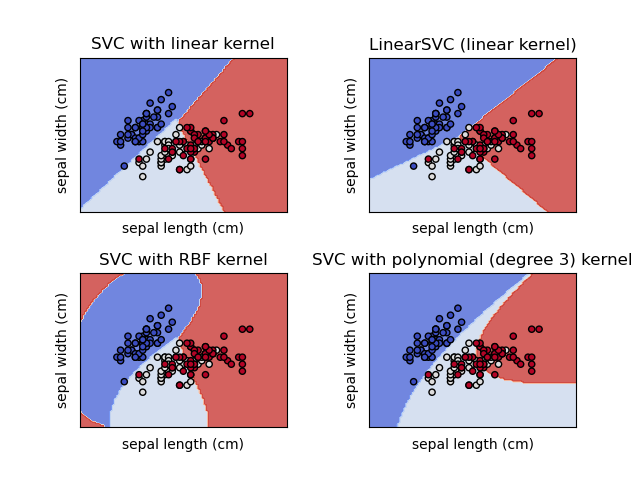
\includegraphics[width=14cm]{figuras/plot-svc.png} 
    \legend{Fonte: \href{https://scikit-learn.org/stable/modules/svm.html}{\cite{scikit_svm_module}} (2022, p. TO-DO)}
    \label{fig:internet} 
\end{figure}

\subsection{Stochastic Gradient Descent}

Gradiente descendente estocástico é um método iterativo para otimização de uma função objetivo com propriedades "suaves" (diferenciais ou subdiferenciais) adequadas. \cite{ruder2016overview}

Pode ser considerada uma aproximação estocástica da otimização por gradiente descendente, uma vez que substitui o gradiente atual (calculado do dataset inteiro) por uma estimativa do mesmo calculada for um subconjunto dos dados selecionado aleatoriamente.
Em problemas de otimização com muitas dimensões, reduz o peso computacional, tendo resultados mais rápidos com o \textit{tradeoff} de perda na taxa de convergência.
O SGD procura encontrar o mínimo global de uma função através de ajustes de configuração a cada tentativa. Ao invés de reduzir o erro ou achar o gradiente para o dataset inteiro, o método reduz o erro através de aproximações em direção ao gradiente para um subconjunto aleatório do dataset, que pode ser tão pequeno quanto o conjunto de dados de treinamento inicial.
De forma heurística, se o modelo inicial erra muito, as alterações na configuração vão tornando o modelo mais preciso. Em contrapartida, é possível que questões antes acertadas, possam passar a serem erradas ou aumento da taxa de erro geral em favor de acertos específicos. Nem toda iteração necessariamente irá fazer o modelo melhorar.
Positivamente, o SGD consegue sair do mínimo local em direção ao mínimo global através dos ajustes de configuração com baixo custo computacional em relação ao gradiente descendente clássico.
\cite{overview_gradient_descent_stochastic}

\begin{figure}[ht]
    \centering
    \caption{Função Objetivo}
    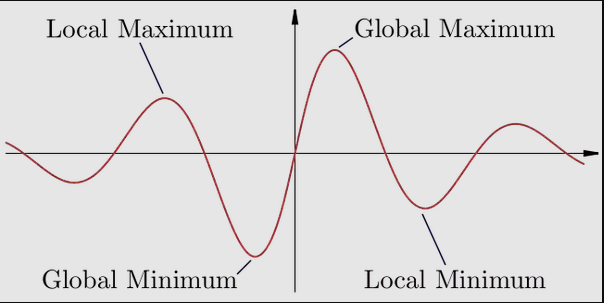
\includegraphics[width=10cm,height=14cm,keepaspectratio]{figuras/funcao_objetivo.png} 
    \legend{Fonte: \href{https://deepai.org/}{Função Objetivo} (2022, p. TO-DO)}
    \label{fig:internet} 
\end{figure}

\includecode[C]{Função de um SGD elementar} {alg:codigo1}{codigos/sgd.py}

\bigskip

\subsection{AdaBoost}

\textit{AdaBoost} é um algoritmo do tipo \textit{Boosting} \cite{wu2011some} com capacidade auto-adaptativa que melhora a performance de classificadores fracos por estabelecer um conjunto de múltiplos classificadores. Como o \textit{AdaBoost} adapta-se a taxa de erro do algoritmo básico em treinamento através de regulação dinâmica do peso de cada amostra, o interesse dos pesquisadores tem sido estimulado.

O método de \textit{Boosting} vem da análise teórica do modelo de aprendizado chamado PAC (\textit{Probably Approximately Correct}). Os autores Kearns e Valiant propuseram os conceitos de aprendizado forte e fraco. No modelo de aprendizado do PAC, se um algoritmo de aprendizado polinomial para identificar um grupo de conceito e a acurácia do reconhecimento é muito alta, esse grupo de conceitos são considerados como aprendizado forte. Porém, se a taxa de corretude do algoritmo de aprendizado de identificação é um pouco superior a tentativa aleatória de adivinhar, então esse grupo é considerado aprendizado fraco. 

Kearns e Valient perceberam uma relação de equivalência entre aprendizado fraco e forte, onde o algoritmo de aprendizado fraco pode ser promovido para aprendizado forte.
Se existe uma equivalência entre fraco e forte, então enquanto aprende-se um conceito, pode-se elevar um algoritmo um pouco melhor que tentativas de adivinhação aleatórias para um algoritmo de aprendizado forte (desde que se saiba qual algoritmo forte em específico).

Em 1990, Schapire publicou o primeiro método de Boosting. Freund fez melhorias e criou um método muito melhor conhecido como BBM (boost-by-majority).
\textit{Boosting} produz uma série de classificadores antes e depois do treinamento. O conjunto de treinamento utilizado em cada classificador é um subconjunto advindo do conjunto geral de treinamento e se cada amostra aparece no subconjunto ou não depende da performance dos classificadores anteriores. No caso das amostras julgadores como incorretas pelos classificadores já existentes, então ã probabilidade de surgirem no novo subconjunto de treinamento será muito maior, fazendo com que os classificadores seguintes tenham foco em lidar com as diferenças nas amostras, que é uma tarefa árdua para os classificadores já existentes.

O método \textit{Boosting} pode aumentar a capacidade de generalização de um dado algoritmo, mas o algoritmo precisa ter estabelecido o limite inferior da acurácia de aprendizagem de um classificador fraco, que na prática é uma tarefa difícil.

\textit{AdaBoost} que surgiu em 1995 atráves de Freund e Schapire fez uma melhoria no algoritmo de \textit{Boosting}.
Sendo o algoritmo mais representativo da família, ele mantém a distribuição de um conjunto de probabilidades para amostras de treinamento e ajusta a probabilidade de distribuição de cada amostra durante a iteração. Um algoritmo específico de aprendizado é usado para gerar o classificador-membro e calcular a taxa de erro nas amostras de treinamento. \textit{AdaBoost} irá usar a taxa de erro para ajustar a probabilidade de distribuição das amostras de treino. O papel de mudar os pesos é para aumentar o impacto das classificações incorretas e reduzir o impacto das classificações corretas. Por fim, com o ajuste dos pesos nos classificadores únicos, é obtido um classificador forte.
O pseudoalgoritmo tem a seguinte estrutura com um conjunto de amostras iniciais:

\begin{equation}
    L=\left\{\left(x_{1}, y_{1}\right),\left(x_{2}, y_{2}\right) \cdots\left(x_{N}, y_{N}\right)\right\}, y_{i} \in\{+1,0\}
\end{equation}

A distribuição inicial dos pesos é dada por:

\begin{equation}
    w_{i}^{1}=\frac{1}{N}
\end{equation}

Onde +1 é uma amostra positiva e 0 é uma amostra negativa, sendo o total de amostras N.

Considerando t = 1, ... , T, tem-se um \textit{loop} com os pesos normalizados:

\begin{equation}
    w_{i}^{t}=\frac{w_{i}^{t}}{\sum_{j=1}^{N} w_{j}^{t}}
\end{equation}

O classificador fraco que seleciona e classifica do conjunto de amostras aquele cuja taxa de erro é a menor e a distribuição do peso atual $h_{t}$. A taxa de erro do classificador fraco é dada pela expressão:

\begin{equation}
    \mathcal{E}_{t}=\sum_{i=1}^{N} w_{i}^{t}\left|h_{t}\left(x_{i}\right)-y_{i}\right|
\end{equation}

A atualização do peso da amostra é dada por:

\begin{equation}
    w_{i}^{t+1}=w_{i}^{t} \beta_{t}^{1-e_{i}}
\end{equation}

$e_{i}$ = 0 representa que xi foi classificado corretamente e $e_{i}$ = 1 significa que $x_{i}$ foi classificado incorretamente.

Como saída final do algoritmo:

\begin{equation}
    \begin{aligned}
    &H(x)= \begin{cases}1, & \sum_{t=1}^{T} \alpha_{t} h_{t}(x) \geq \frac{1}{2} \sum_{t=1}^{T} \alpha_{t} \\ 0, & \text { caso contrario }\end{cases}\\
    &\alpha_{t}=\log \frac{1}{\beta_{t}} .
    \end{aligned}
\end{equation}

